%-----------------------------------------------------------------
%	BASIC DOCUMENT LAYOUT
%-----------------------------------------------------------------
\documentclass[paper=a4, fontsize=12pt, twoside=semi, abstracton, listof=totoc, toc=left]{scrartcl}
\usepackage[T1]{fontenc}
\usepackage[utf8]{inputenc}
\usepackage{lmodern}
\usepackage{slantsc}
\usepackage{microtype}
\usepackage[british]{babel}
% \usepackage[backend=bibtex, style=phys, sorting=none, citestyle=authoryear, maxbibnames=3, maxcitenames=2]{biblatex}
\usepackage[backend=bibtex, style=trad-abbrv, sorting=none, maxbibnames=3, maxcitenames=2]{biblatex}
\addbibresource{bibliography.bib}
% \bibliographystyle{apalike}
\makeatletter
	\def\blx@maxline{77}
\makeatother

% Sectioning layout
\addtokomafont{sectioning}{\normalfont\scshape}
\usepackage{tocstyle}
\usetocstyle{standard}
\renewcommand*\descriptionlabel[1]{\hspace\labelsep\normalfont\bfseries{#1}}
\usepackage[titletoc]{appendix}

% Empty pages
\usepackage{etoolbox}
% \pretocmd{\toc}{\cleardoubleevenemptypage}{}{}
\pretocmd{\section}{\cleardoubleevenemptypage}{}{}
% \pretocmd{\section}{\clearpage}{}{}
\pretocmd{\part}{\cleardoubleevenemptypage\thispagestyle{empty}}{}{}
\renewcommand\partheadstartvskip{\clearpage\null\vfil}
\renewcommand\partheadmidvskip{\par\nobreak\vskip 20pt\thispagestyle{empty}}

% Paragraph indentation behaviour
\setlength{\parindent}{0pt}
\setlength{\parskip}{0.3\baselineskip plus2pt minus2pt}
\newcommand{\sk}{\medskip\noindent}

% Fancy header and footer
\usepackage{fancyhdr}
\pagestyle{fancyplain}
\fancyhead[LO]{\thepage}
\fancyhead[CO]{}
\fancyhead[RO]{\nouppercase{\mytitle}}
\fancyhead[LE]{\nouppercase{\rightmark}}
% \fancyhead[LE]{\nouppercase{\leftmark}}
\fancyhead[CE]{}
\fancyhead[RE]{\thepage}
\fancyfoot{}
\renewcommand{\headrulewidth}{0.3pt}
\renewcommand{\footrulewidth}{0pt}
\setlength{\headheight}{13.6pt}

%-----------------------------------------------------------------
%	MATHS AND SCIENCE
%-----------------------------------------------------------------
\usepackage{amsmath,amsfonts,amsthm,amssymb}
\usepackage{xfrac}
\usepackage[a]{esvect}
\usepackage{chemformula}
% For plotting block diagrams
\usepackage{tikz}
\usetikzlibrary{shapes,arrows}
\usepackage{graphicx}
	\graphicspath{{images/}}

% Theorem environment	
\usepackage{amsthm}
\newtheorem{mydef}{Definition}
\newtheorem{myprop}{Proposition}
\newtheorem{mythm}{Theorem}
\newtheorem{mylem}{Lemma}
\newtheorem{mycor}{Corollary}
\newtheorem{myrem}{Remark}

\usepackage[arrowdel]{physics}
	\renewcommand{\vnabla}{\vec{\nabla}}
	% \renewcommand{\vectorbold}[1]{\boldsymbol{#1}}
	% \renewcommand{\vectorarrow}[1]{\vec{\boldsymbol{#1}}}
	% \renewcommand{\vectorunit}[1]{\hat{\boldsymbol{#1}}}
	\renewcommand{\vectorarrow}[1]{\vec{#1}}
	\renewcommand{\vectorunit}[1]{\hat{#1}}
	\renewcommand*{\grad}[1]{\vnabla #1}
	\renewcommand*{\div}[1]{\vnabla \vdot \va{#1}}
	\renewcommand*{\curl}[1]{\vnabla \cp \va{#1}}
	\let\rot\curl

% SI units
\usepackage[separate-uncertainty=true]{siunitx}
% \sisetup{range-phrase = \text{--}, range-units = brackets}
\sisetup{range-phrase = \text{--}, range-units = single}
\DeclareSIPrePower\quartic{4}
	%\DeclareSIUnit\micron{\micro\metre}

% Smaller trig functions
\newcommand{\Sin}{\trigbraces{\operatorname{s}}}
\newcommand{\Cos}{\trigbraces{\operatorname{c}}}
\newcommand{\Tan}{\trigbraces{\operatorname{t}}}
\DeclareMathOperator{\Det}{det}
\DeclareMathOperator{\im}{im}
\DeclareMathOperator{\Rank}{rank}
\DeclareMathOperator{\Deg}{deg}

% Operator-style notation for matrices
\newcommand*{\mat}[1]{\hat{#1}}

% Matrices in (A|B) form via [c|c] option
\makeatletter
\renewcommand*\env@matrix[1][*\c@MaxMatrixCols c]{%
  \hskip -\arraycolsep
  \let\@ifnextchar\new@ifnextchar
  \array{#1}}
\makeatother

% Shorter \mathcal and \mathbb
\newcommand*{\mc}[1]{\mathcal{#1}}
\newcommand*{\mbb}[1]{\mathbb{#1}}

% Shorter ^\ast and ^\dagger
\newcommand*{\sast}{^{\star}{}}
\newcommand*{\sdag}{^{\dagger}{}}

% Blackboard bold identity
\usepackage{bbm}
\newcommand*{\bbid}{\mathbbm{1}}

% Shorter displaystyle
\newcommand*{\dsp}{\displaystyle}

% Inexact differential
\newcommand{\dbar}{\mathchar'26\mkern-12mu\mathrm{d}}
\newcommand{\indd}[1]{\dbar{#1}}

% Arrows with text and cancels for developments
\newcommand{\tikzmark}[1]{\tikz[overlay,remember picture] \node (#1) {};}
\tikzset{square arrow/.style={to path={-- ++(0,-.25) -| (\tikztotarget)}}}
\usepackage{cancel}

\newcommand*\acr[1]{\textscale{.85}{#1}}

%-----------------------------------------------------------------
%	OTHER PACKAGES
%-----------------------------------------------------------------
\usepackage{environ}

%Left numbered equations
\makeatletter
	\NewEnviron{Lalign}{\tagsleft@true\begin{align}\BODY\end{align}}
\makeatother

% Plots and graphics
\usepackage{pgfplots}
\usepackage{tikz}
\usepackage{color}
	\makeatletter
		\color{black}
		\let\default@color\current@color
	\makeatother

% Richer enumerate, figure, and table support
\usepackage{enumerate}
\usepackage[shortlabels]{enumitem}
\usepackage{float}
\usepackage{subfig}
% \usepackage{subcaption}
\usepackage{tabularx}
\usepackage{booktabs}
	%\setlength{\intextsep}{8pt}
% \numberwithin{equation}{section}
% \numberwithin{figure}{section}
% \numberwithin{table}{section}
% \counterwithin{lstlisting}{section}

% No indentation after certain environments
\makeatletter
\newcommand*\NoIndentAfterEnv[1]{%
	\AfterEndEnvironment{#1}{\par\@afterindentfalse\@afterheading}}
\makeatother
%\NoIndentAfterEnv{thm}
\NoIndentAfterEnv{defi}
\NoIndentAfterEnv{example}
\NoIndentAfterEnv{table}

% Misc packages
\usepackage{ccicons}
\usepackage{lipsum}
\usepackage{todonotes}
\usepackage{array}
\usepackage{multirow}

% Print DOI only if there's no URL
\renewbibmacro*{doi+eprint+url}{%
  \iftoggle{bbx:doi}
    {\iffieldundef{url}{\printfield{doi}}{}}
    {}%
  \newunit\newblock
  \iftoggle{bbx:eprint}
    {\usebibmacro{eprint}}
    {}%
  \newunit\newblock
  \iftoggle{bbx:url}
    {\usebibmacro{url+urldate}}
    {}}

%-----------------------------------------------------------------
%	SYNTAX HIGHLIGHTING
%-----------------------------------------------------------------
\usepackage[formats]{listings}
\usepackage{relsize}
\usepackage{chngcntr}

\renewcommand{\lstlistingname}{Snippet}
\renewcommand{\lstlistlistingname}{List of snippets}

\lstloadlanguages{python,matlab}

\newcommand*{\inline}{\lstinline[basicstyle=\normalsize\ttfamily]}


\lstset{language=matlab,
		frame=tb,
		% captionpos=b,
		tabsize=2,
		% showtabs=true,
		breaklines=true,
		breakatwhitespace=true,
		basicstyle=\smaller\ttfamily,
		numbers=left,
		numberstyle=\tiny,
		numbersep=7.5pt,
		% commentstyle=\textsl,
		xleftmargin=3ex}
\lstset{escapeinside={(*}{*)}}   % for (*\ref{ }*) inside lstlistings (Scode)

\lstdefinestyle{output}{
	language=,
	% showtabs=true,
	% showspaces=true,
	numbers=none,
	frame=tblr,
	% columns=fullflexible,
	% backgroundcolor=\color{blue!10},
	numbers=none,
	xleftmargin=3ex}

\expandafter\patchcmd\csname \string\lstinline\endcsname{%
	\leavevmode
	\bgroup
}{%
	\leavevmode
	\ifmmode\hbox\fi
	\bgroup
}{}{%
	\typeout{Patching of \string\lstinline\space failed!}%
}
%% end of patch

%-----------------------------------------------------------------
%	THEOREMS
%-----------------------------------------------------------------
\usepackage{thmtools}

% Theroems layout
\declaretheoremstyle[
	spaceabove=6pt, spacebelow=6pt,
	headfont=\normalfont,
	notefont=\mdseries, notebraces={(}{)},
	bodyfont=\small,
	postheadspace=1em,
]{small}

\declaretheorem[style=plain,name=Theorem,qed=$\square$,numberwithin=section]{thm}
\declaretheorem[style=plain,name=Corollary,qed=$\square$,sibling=thm]{cor}
\declaretheorem[style=plain,name=Lemma,qed=$\square$,sibling=thm]{lem}
\declaretheorem[style=definition,name=Definition,qed=$\blacksquare$,numberwithin=section]{defi}
\declaretheorem[style=definition,name=Example,qed=$\blacktriangle$,numberwithin=section]{example}
\declaretheorem[style=small,name=Proof,numbered=no,qed=$\square$]{sproof}

%-----------------------------------------------------------------
%	DEDICATION ENVIRONMENT
%-----------------------------------------------------------------

\newenvironment{mydedication}
	{\clearpage           % we want a new page
	\thispagestyle{empty}% no header and footer
	\vspace*{\stretch{1}}% some space at the top
	\itshape             % the text is in italics
	\raggedleft          % flush to the right margin
	}
	{\par % end the paragraph
	\vspace{\stretch{3}} % space at bottom is three times that at the top
	\clearpage           % finish off the page
	}

%-----------------------------------------------------------------
%	PDF INFO AND HYPERREF
%-----------------------------------------------------------------
\usepackage{hyperref}
\hypersetup{colorlinks, citecolor=black, filecolor=black, linkcolor=black, urlcolor=black}
\usepackage{cleveref}
	\crefname{section}{\S}{\SS}
	\Crefname{section}{\S}{\SS}
	\crefname{listing}{snippet}{}

\newcommand*{\mytitle}{Modelling Trailer Parking}
\newcommand*{\mysubtitle}{}
\newcommand*{\myauthor}{Alfredo Hernández \and David Masip \and Martí Municoy \and Jan-Hendrik Niemann}
\newcommand*{\myuni}{Universitat Autònoma de Barcelona}
% \newcommand*{\mydate}{12th December 2017}
\newcommand*{\mydate}{2nd February 2018} % Deadline

\pdfstringdefDisableCommands{\def\and{and }}

\usepackage{hyperxmp}
\hypersetup{pdfauthor={\myauthor}, pdftitle={\mytitle: \mysubtitle}}

%-----------------------------------------------------------------
%	TITLE SECTION AND DOCUMENT BEGINNING
%-----------------------------------------------------------------
\newcommand{\horrule}[1]{\rule{\linewidth}{#1}}
\title{
	\normalfont
	\small \scshape{\myuni} \\ [25pt]
	\horrule{0.5pt} \\ [0.4cm]
	\huge \mytitle \\
% 	\Large \scshape{\mysubtitle} \\
	\horrule{2pt} \\ [0.5cm]
}
\author{\myauthor}
% \\ \footnotesize Supervised by: \mysupervisor \\ \footnotesize Academic tutor: \mytutor}
\date{\today}

\begin{document}

\clearpage\maketitle
\thispagestyle{empty}
\addtocounter{page}{-1}

%-----------------------------------------------------------------
%	DEDICATION
%-----------------------------------------------------------------
% \begin{mydedication}
% 	Dedicated to RMT, Val \& the Brotherhood
% \end{mydedication}

%-----------------------------------------------------------------
%	DOCUMENT BODY
%-----------------------------------------------------------------
\cleardoubleevenemptypage
%-----------------------------------------------------------------
%	ABSTRACT
%	!TEX root = ./../main.tex
%-----------------------------------------------------------------
\cleardoubleevenemptypage
\thispagestyle{empty}
\phantomsection
\addcontentsline{toc}{section}{Abstract}
\begin{abstract}
	The interesting aspect of car-trailer system is that the motion control while moving forward is stable, while reversing the motion is unstable. In this report the system is studied to analyse its stability and how to control it. Based on Classical Control Theory a first model is constructed using linear controller design (programmed in MATLAB). A second model is optimisation-based control (programmed in C). Last but not least, a model is constructed using steering-based control (programmed in Python). It is shown that two of the methods are viable options for control with their own advantages and disadvantages.
\end{abstract}


% \cleardoubleemptypage
\pdfbookmark[1]{\contentsname}{toc}
\tableofcontents

%-----------------------------------------------------------------
%	THE PROBLEM
%	!TEX root = ./../main.tex
%-----------------------------------------------------------------
\section{The Problem}

\subsection{Introduction}
Backing up a car can sometimes be a stressful experience. When you have something attached to your car, it gets even more nerve-racking. The problem is that the motion control while moving forward is stable, while reversing the motion is unstable. We want to analyse and solve this problem using mathematical and physical concepts.

To tackle this problem, we need to create a model of the system using differential equations and then design a controller for the system, that is, a mathematical model that can modify dynamically the behaviour of the system to follow a control or reference trajectory.

\begin{figure}[H]
    \centering
    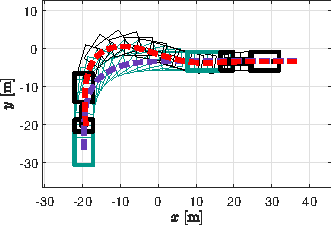
\includegraphics[width=0.55\textwidth]{images/trailer-diagram2}
    \caption{Traversed paths by the car (red line) and the trailer (purple line)}
    \label{fig:trailer-diagram2}
\end{figure}

In short, using figure \ref{fig:trailer-diagram2} as a reference, we would like to predict and control the trajectory purple dashed line (trajectory of the trailer) whilst only having direct access to the physical system that controls the red line (trajectory of the car).

%-----------------------------------------------------------------
\subsection{Modelling the Kinematics}\label{sec:kinematics}
\label{kinem}
Before thinking on the model, we need to make some initial assumptions to simplify the problem. These are the initial assumptions we thought they will ease the modelling work: 
% \begin{itemize}
%     \item The system has a unique pivoting point: the hitch.
%     \item The ground is flat.
%     \item The system is slip free.
%     \item The car backs at constant velocity.
%     \item The trailer's mass is uniformly distributed.
%     \item The trailer has a single-axle.
% \end{itemize}

\begin{itemize}
    \item The system has a unique pivoting point, the hitch. This is completely necessary because it is the responsible of yielding this unstable equilibrium point when driving backwards. 
    \item We assume a flat, nonslippery ground. 
    \item The velocity of the car will be constant when going backwards. Given a steering angle, the car follows a
    circular path.
    \item As we want to work with a geometric model, we need the effect of the mass distribution to be negligible, so we assume a trailer with a uniformly distributed mass. 
    \item Finally, we will work with a trailer that only has a single axle for the wheels.
\end{itemize}

Considering these assumptions, we can focus on the model. We chose a geometric model which only looks at the rate at which the $\phi$ angle changes along time. So our main goal is to predict the $\phi$ angle along the trajectory of the car. 

Figure \ref{fig:geom-model} shows the model of the vehicle-trailer system, and the parameters of the model are presented in table \ref{tab:parameters} below.
\begin{figure}[H]
    \centering
    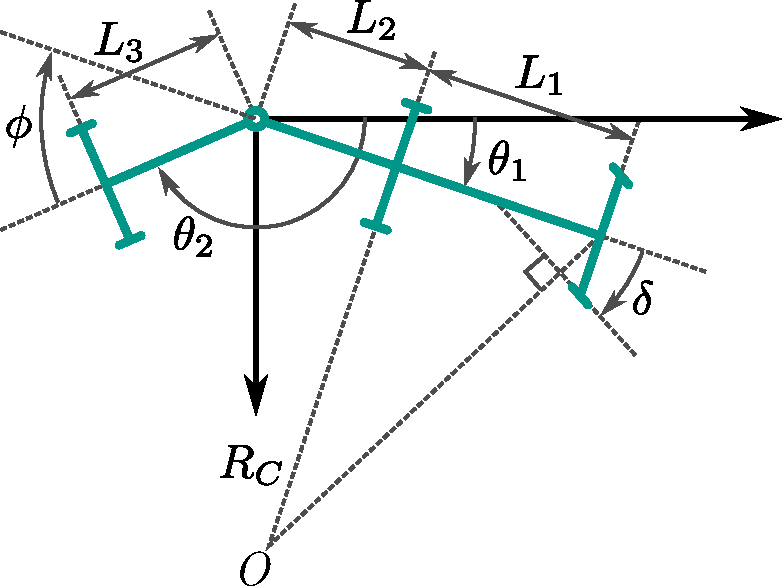
\includegraphics[width=0.5\textwidth]{images/trailer-diagram}
    \caption{Geometric model of the car-trailer system}
    \label{fig:geom-model}
\end{figure}

\begin{table}[H]
    \centering
    \begin{tabularx}{0.95\textwidth}{c X}
        \toprule
        \toprule
        System parameters & Description \\
        \midrule
        $\theta_{1}$  & The angle the car is travelling at with respect to a global coordinate system. \\
        $\theta_{2}$  & The angle the trailer is travelling at with respect to a global coordinate system. \\
        $\phi$        & The angle between the car and the trailer. \\
        $\delta$      & The steering angle of the vehicle's wheels. \\
        $V$           & Reversing speed of the car. \\
        $V_{trailer}$ & Reversing speed of the trailer. \\
        $R_{C}$       & Distance from the centre of rotation $O$ to the rear axle of the car. \\
        $L_{1}$       & Wheelbase of the car. \\
        $L_{2}$       & Overhang from the rear axle of the car to the hitch point. \\ 
        $L_{3}$       & Distance from the trailer axle to the hitch. \\ 
        \bottomrule
    \end{tabularx}
    \caption{Physical parameters of the system described by our model}
    \label{tab:parameters}
\end{table}

If we know $\phi$, we will be able to predict the trajectory of the trailer. The angle $\phi$ is defined as
\begin{align}
    \phi = \pi - (\theta_{2} - \theta_{1}) ,
\end{align}
where $\theta_{2}$ and $\theta_{1}$ are the angles belonging to the car and to the trailer, expressed according to one reference axle. 

Taking the derivative of the angle $\phi$, we obtain
\begin{align}\label{eq:dphi}
    \dot{\phi} = -\dot{\theta}_{2} + \dot{\theta}_{1} ,
\end{align}

Using the distance to the centre of rotation $O$ from the cars' rear axis, an expression for the angular velocity of the car is obtained:
\begin{align}\label{eq:dtheta1-0}
    \dot{\theta}_{1} = -\frac{V}{R_{C}} .
\end{align}
This is, of course, because given a $\delta$, the car follows a uniform circular path. This is what is usually known as Ackerman kinematics (see \cite{steering}), which state that, for a given $\delta$,
every point of the car follows a concentric circular path. The 
centre of these circles can be computed using trigonometry.\\

Using Ackerman kinematics, we can compute the angular velocity as the ratio of the longitudinal speed and the
radius of the path. We can compute the radius of the path using trigonometry, and we obtain:
\begin{align*}
    R_C = \frac{\tan \delta}{L_1}
\end{align*}

Joining the two last expressions we can obtain the following expression:
\begin{align}\label{eq:dtheta1}
    \dot{\theta}_{1} = -\frac{V}{L_{1}} \tan \delta . \tag{\ref{eq:dtheta1-0} bis}
\end{align}

%It is the rate of change of $\theta_{1}$ along time and it depends on the velocity of the car, $V$, the distance between both wheel axles of the car, $L_{1}$, and the angle of the front wheels, $\delta$.

To predict $\phi$, we also need to know how $\theta_{2}$ varies along time. For this reason, we need to know which is the longitudinal speed and the normal speed at the point that joins the car and the trailer. Of course, the longitudinal speed is $V$, and, as the car is rotating at angular velocity $\dot{\theta}_{1}$, the normal speed of that point is $L_2\cdot\dot{\theta}_{1}$. We can compute the longitudinal speed of the trailer by projecting in the longitudinal axis of the trailer the normal and longitudinal speed of the car in the point than joins them:
\begin{align}
    V_{trailer} = -L_{2} \dot{\theta}_{1} \sin \phi + V \cos \phi .
\end{align}
We can also compute the normal speed by projecting the longitudinal and normal speeds in the normal direction of the trailer. This normal speed will be $L_3\dot{\theta_2}$. 
Using this, $\dot{\theta}_{2}$ can be isolated:
\begin{align}\label{eq:dtheta2}
    \dot{\theta}_{2} =  \frac{L_{2} \dot{\theta}_{1} \cos \phi + V \sin \phi }{L_{3}} .
\end{align}

Replacing \eqref{eq:dtheta1} and \eqref{eq:dtheta2} into \eqref{eq:dphi}, we get the variation of $\phi$ along time. It is expressed in terms of the velocity of the car, the distance between the hitch and the trailer axle, the distance between the rear car axle and its hitch, the distance between both wheel axles for the car and the angle of the car’s front wheels:
\begin{align}\label{eq:dotphi-final}
    \dot{\phi} = - \frac{V}{L_{3}} \sin \phi - \frac{V}{L_{1}} \tan \delta \qty( 1 + \frac{L_{2}}{L_{3}} \cos \phi ) .
\end{align}
Of course, this system assumes that $V>0$ when the car is going backwards. As all the geometric arguments are valid, if we take $V < 0$, we will obtain the dynamics of the trailer when the car is going forward.

Here we observe that if we set $\delta = 0$, then the differential equation becomes
\begin{align}\label{eq:dotphi-final-bis}
    \dot{\phi} = - \frac{V}{L_{3}} \sin \phi . \tag{\ref{eq:dotphi-final} bis}
\end{align}

In this case, $\phi = 0$ is a critical point of the differential equation. To analyse its stability, we have to discuss the sign of:
\begin{align}\label{eq:stability-0}
    \dv{\phi} \qty( - \frac{V}{L_{3}} \sin \phi )  = - \frac{V}{L_{3}} \cos \phi
\end{align}
at the critical point. At $\phi = 0$, the previous expression becomes
\begin{align}\label{eq:stability}
    -\frac{V}{L_3} . \tag{\ref{eq:stability-0} bis}
\end{align}
This shows that when $V > 0$ (car going backwards) this critical point is unstable, and when $V < 0$ the point is stable.

\bigskip
In the simulation, we will also take into account the phenomenon of jackknifing. A trailer jackknifes when its $\phi$
angle grows up to the point where the trailer contacts the car.
Of course, by all means we want to avoid this situation. As a general fact accepted in the bibliography, (see \cite{jack}) when $\phi$ surpasses a critical $\phi_{crit}$, the trailer cannot be controlled and the jackknifing phenomenon occurs.

\bigskip
We have already derived a model for the kinematics of the trailer with respect to the movement of the car. In order to produce a proper simulation of the whole system, we need to model the kinematics of the car as well. The model that we have used is based on Ackerman kinematics. The result of the model is that every point of the car moves through a circular path of centre $O$ (see Figure \ref{fig:geom-model}).


%-----------------------------------------------------------------
\subsection{Controller Design}

We think that our problem is mainly a control theory based problem. The aim is to design a controller for the system to drive the state $\phi$ to the wished state by changing the steering angle $\delta$. We would like to consider a linear controller which applies to the nonlinear model. The following section gives a mathematical introduction on control theory and afterwards the controller is presented.

%-----------------------------------------------------------------
%	CONTROL THEORY
%	!TEX root = ./../main.tex
%-----------------------------------------------------------------
\section{Mathematical Systems and Control Theory}\label{sec:intro-msct}

The following section deals with the topic of mathematical control theory. A short introduction is given, followed by a discussion of selected terms and definitions needed for this work. Among other things the term \emph{controllability} and the \emph{pole placement theorem} will be presented. We will only see the relevant proofs. All omitted proofs can be found in \cite{Sontag1998, Hinrichsen2005, Hautus2001}.\footnote{If you are familiar with this topic you can skip this section and continue with \cref{sec:controllerdesign}}\\

Classical techniques for analysis and design of control systems have been used for more than five decades in a vast variety of industrial applications. These methods are based on transfer function models of the plant to be controlled. However, when it comes to more evolved tasks with e.g. more input and output variables other techniques are used. These techniques are based on state space models of the plant. One major advantage of state space models is for example that single-input single-output systems are equally treated as multi-input multi-output systems.

\tikzstyle{block} = [draw, fill=white, rectangle,
minimum height=3em, minimum width=6em]
\tikzstyle{sum} = [draw, fill=white, circle, node distance=1cm]
\tikzstyle{input} = [coordinate]
\tikzstyle{output} = [coordinate]
\tikzstyle{pinstyle} = [pin edge={to-,thin,black}]

\begin{figure}[H]
	\centering
	% The block diagram code is probably more verbose than necessary
	\begin{tikzpicture}[auto, node distance=4cm,>=latex']
	% We start by placing the blocks
	\node [input, name=input] {};
	%\node [sum, right of=input] (sum) {};
	%\node [block, right of=input] (controller) {Controller};
	\node [block, right of=input,node distance=4cm] (system) {Dynamical System};
	% We draw an edge between the controller and system block to
	% calculate the coordinate u. We need it to place the measurement block.
	\draw [->] (input) -- node[name=u] {$u$} (system);
	\node [output, right of=system] (output) {};
	%\node [block, below of=u] (measurements) {Measurements};

	% Once the nodes are placed, connecting them is easy.
	%\draw [draw,->] (input) -- node {$r$} (sum);
	%\draw [->] (sum) -- node {$e$} (controller);
	\draw [->] (system) -- node [name=y] {$y$}(output);
	%\draw [->] (y) |- (measurements);
	%\draw [->] (measurements) -| node[pos=0.99] {$-$}
	%node [near end] {$y_m$} (sum);
	\end{tikzpicture}
	\caption{Block diagram of a dynamical system}
	\label{fig:blockdiagram_dyn_sys}
\end{figure}

For this work we consider a dynamical system which can be represented by a block diagram as seen in figure \ref{fig:blockdiagram_dyn_sys}. There is an input $u(t)$ which represents controls, noises and disturbances and an output $y(t)$ representing the measurements. We assume that the behaviour of this “black box” can be approximated by the mathematical model
\begin{align}\label{eq:dynsys}
	\begin{split}
		\dot{x}(t) &= f(t, x(t), u(t))\\
		\dot{y}(t) &= h(x(t), u(t))
	\end{split}
\end{align}
were $x$ is the vector of internal variables. When modelling a physical system, $x$ is not necessary related to the “real” physical variables.

We consider that system (\ref{eq:dynsys}) is a linear system of the form
\begin{align*}
	\dot{x}(t) &= Ax(t) + Bu(t)\\
	\dot{y}(t) &= Cx(t) + Du(t)
\end{align*}
which is called \emph{linear time-invariant control system} (LTI). The matrices are called \emph{system matrix} $A$, \emph{input matrix} $B$, \emph{output matrix} $C$ and \emph{feed-through matrix} $D$. The class of LTI systems is a very simple class. Nevertheless, lots of processes can be described using this class by a “sufficiently good” linearisation. Nowadays linear models are still used to model “real world” applications. It can be used to approximate the system in a neighbourhood of certain points. This model is obtained by linearisation which is feasible at points $(x^*,u^*)$ such that $f(x^*,u^*) = 0$. These points are equilibrium points.

%-----------------------------------------------------------------
\subsection{Controllability}

This section will introduce one important property of linear systems that determine whether or not given control objectives can be achieved. Simply said, a system is said to be controllable if it is possible to find a control input that takes the system from any initial state to any final state in any given time interval. We will see necessary and sufficient conditions for controllability.

\bigskip
Consider a system in state space realisation
\begin{align}
	\dot{x}(t) &= Ax(t) + Bu(t),\qquad x(t_0) = x^0 \label{eq:IVP}
\end{align}
where $A\in\mathbb{R}^{n\times n}$, $B\in\mathbb{R}^{n\times m}$, $(t_0,x^0)\in\mathbb{R}\times\mathbb{R}^n$, and $u(\cdot) \in U := \mathcal{L}_{loc}^1$. System (\ref{eq:IVP}) will shortly be represented as $(A,B)$. The space of input functions is defined as
\begin{align*}
	\mathcal{L}_{loc}^1 := \{&f:\mathbb{R}\rightarrow\mathbb{R}^m \mid f_i \quad\text{measureable}\\
	&\text{and} \int_K \mid f_i(t)\mid dt < \infty , \quad \forall K \subseteq \mathbb{R} \quad \text{compact}, \quad i=1,...,m  \}.
\end{align*}
Alternatively, the space of input functions $U$ can be defined as $U := \mathcal{PC}(\mathbb{R}\rightarrow\mathbb{R}^m)$ which are all piece-wise continuous functions. An important property of the input space is that $U$ is closed under certain cencatenation, i.e. for any $u_1,u_2\in U$ and $b \in \mathbb{R}$ the concatenation
\begin{align*}
	u_1 \quad\&_b\quad u_2 := \left(t \mapsto
	\begin{cases}
		u_1(t), \quad t \le b\cr
		u_2(t), \quad t > b
	\end{cases} \right)
\end{align*}
is in $U$.

\noindent The unique global solution of the initial value problem (\ref{eq:IVP}) is
\begin{align*}
	t \mapsto x(t;t_0,x^0,u) = e^{A^{(t-t_0)}}x^0 + \int_{t_0}^t e^{A^{(t-s)}}Bu(s)ds.
\end{align*}
The set of pairs $(x,u)$ which solve (\ref{eq:IVP}) for some $(t_0,x^0)$ is called the \emph{behaviour} of (\ref{eq:IVP}):
\begin{align*}
	\mathcal{B}_{(A,B)} := \{(x,u) \in X\times U\mid \exists (t_0,x^0) \in \mathbb{R}\times\mathbb{R}^n,\quad x(\cdot) = x(\cdot;t_0,x^0,u )    \}
\end{align*}
Here, $X$ is a suitable space of functions such that
\begin{align*}
	\{x(\cdot;t_0,x^0,u ) \mid (t_0,x^0) \in \mathbb{R}\times\mathbb{R}^n, \quad u \in U  \} \subseteq X.
\end{align*}
First, we will define the terms  \emph{reachable}, \emph{controllable} and \emph{null-controllable}.
\begin{mydef}
	A system $(A,B)$ is called
	\begin{itemize}
		\item \emph{Reachable} at time $T > 0$ if for all $x^1 \in \mathbb{R}^n$ there exists $(x,u)\in\mathcal{B}_{(A,B)}$ such that $x(0) = 0$ and $x(T) = x^1$,
		\item \emph{Controllable} at time T if for all $x^0,x^1 \in \mathbb{R}^n$ there exists $(x,u)\in\mathcal{B}_{(A,B)}$ such that $x(0) = x^0$ and $x(T) = x^1$,
		\item \emph{Null-controllable} at time T if for all $x^0 \in \mathbb{R}^n$ there exists $(x,u)\in\mathcal{B}_{(A,B)}$ such that $x(0) = x^0$ and $x(T) = 0$.
	\end{itemize}
\end{mydef}
\noindent Simply said: \emph{Reachable} means that we can steer the system from 0 to any final state in any time $Z$. \emph{Controllable} mean that it is possible to steer the system from any initial state to any final state in any given time $T$ and hence \emph{null-controllable} means that the final state is 0. One easily checks that $x^0 \in\mathbb{R}^n$ is null-controllable at $T$ if and only if there exists a $u\in U$ such that $e^{AT}x^0 + \int_{0}^T e^{A^(T-s)}Bu(s)ds = 0$. This is equivalent to: $-e^{AT}x^0$ is reachable at time $T$.
Next, we define the \emph{reachable set} and the \emph{controllable set}.
\begin{mydef}
	The \emph{reachable set} from $x^0 \in \mathbb{R}^n$ at time $T>0$ is defined as
	\begin{align*}
		\mathcal{R}_{x^0}(T) := \{x^1 \in \mathbb{R}^n \mid \exists (x,u) \in \mathcal{B}_{(A,B)}: x(0) = x^0, x(T) = x^1   \}.
	\end{align*}\\The \emph{controllable set} to $x^1\in\mathbb{R}^n$ at time $T$ is defined as
	\begin{align*}
		\mathcal{C}_{x^1}(T) := \{x^0 \in \mathbb{R}^n \mid \exists (x,u) \in \mathcal{B}_{(A,B)}: x(0) = x^0, x(T) = x^1   \}.
	\end{align*}
\end{mydef}
Having this definition we can make the following proposition.
\begin{myprop}\label{prop:2.4}
	For $(A,B)$ we have $\mathcal{R}_0(T) = e^{AT}\mathcal{C}_0(T)$ and, in particular, $(A,B)$ is reachable at time $T$ if and only if $(A,B)$ is null controllable at time $T$.
\end{myprop}
\noindent From Proposition \ref{prop:2.4} we can deduce the following.
\begin{myprop}
	The system $(A,B)$ is reachable at $T>0$ if and only if $(A,B)$ is null-controllable at $T>0$ if and only if $(A,B)$ is controllable at $T>0$.
\end{myprop}
\begin{proof}
	By Proposition \ref{prop:2.4} it only remains to prove that if $(A,B)$ is reachable at $T$ then $(A,B)$ is controllable at $T$.\\Let $x^0,x^1 \in\mathbb{R}^n$ be reachable at time $T$. Then there exists $(x_1,u_1) \in \mathcal{B}_{(A,B)}$ such that $x_1(0)=0$ and $x_1(T)=x^0$ and there exists $(x_2,u_2)\in\mathcal{B}_{(A,B)}$ such that $x_2(0) = 0$ and $x_2(T) = x^1-x_1(2T)$. Since $(x_1(\cdot + T), u_1(\cdot+T)  )\in\mathcal{B}_{(A,B)}$, which is known as \emph{shift-invariance} of the behaviour, we find
	\begin{align*}
		(x(\cdot),u(\cdot)) := (x_1(\cdot+T)+x_2(\cdot), u_1(\cdot+T) +u_2(\cdot)  ) \in \mathcal{B}_{(A,B)}
	\end{align*}
	with
	\begin{align*}
		x(0) &= x_1(T) + x_2(0) = x^0\\
		x(T) &= x_1(2T) + x^1-x_1(2T) = x^1.
	\end{align*}
\end{proof}
In general it is hard to check if for any $x^0,x^1\in\mathbb{R}^n$ there exists an input $u$ that steers $x^0$ to $x^1$. To check this easily the following helps.
\begin{mythm}\label{thm:2.7}
	For all $T>0$ it holds
	\begin{align*}
		\mathcal{R}_0(T) = \im[B,AB,...,A^{n-1}B]   =: \im K(A,B) \in \mathbb{R}^{n \times nm}.
	\end{align*}
\end{mythm}
The matrix $K$ is known as the \emph{Kalman}-matrix. To proof this theorem we need the following lemma.
\begin{mylem}\label{lem:2.8}
	For any $\eta\in\mathbb{R}^n$ and system $(A,B)$ the following conditions are equivalent:
	\begin{enumerate}
		\item \label{1} $\eta$ is orthogonal to the reachable set $\mathcal{R}_0(T)$
		\item \label{2} For all $t\in [0,T]$ it holds $\eta^Te^{At}B=0$
		\item \label{3} For all $k \in \mathbb{N}_0$ it holds $\eta^TA^kB=0$
		\item \label{4} $\eta^T[B,AB,...,A^{n-1}B] = 0$.
		\end{enumerate}
\end{mylem}
\begin{proof}
	First we show that \ref{1} implies \ref{2}.\\Let $x^1 \in \mathcal{R}_0(T)$ Then $x^1=\int_0^Te^{A(T-s)}Bu(s)ds$ for some input $u\in U$. Since $\eta^Tx^1 = 0$ it follows that for all inputs $u\in U$ we have
	\begin{align*}
		\eta^T \int_0^Te^{A(T-s)}Bu(s)ds = 0.
	\end{align*}
	For $u(\cdot) = B^Te^{A^T(T-s)}\eta \in U$ we find
	\begin{align*}
		\int_0^T \eta^Te^{A(T-s)}BB^Te^{A^T(T-s)}\eta ds = 0
	\end{align*}
	which is equivalent to
	\begin{align*}
		\int_0^T \mid\mid   B^Te^{A^T(T-s)}\eta\mid\mid^2 ds \ge 0.
	\end{align*}
	Therefore, for all $s \in [o,T]$ we have $B^Te^{A^T(T-s)}\eta = 0$.\\Now we will show that \ref{2} implies \ref{1}.\\Let $x^1\in\mathcal{R}_0(T)$. Then there exists $u\in U$ so that
	\begin{align*}
		\eta^Tx^1 = \eta^T\int_0^Te^{A(t-s)}Bu(s)ds = 0
	\end{align*}
	which implies that $\eta$ is orthogonal to $\mathcal{R}_0(T)$.\\Next we will show that \ref{2} implies \ref{3}.\\For $t=0$ we have $\eta^TB=0$. Therefore, for all $t\in [0,T]$ we have
	\begin{align*}
		0 &= (\frac{d}{dt})^k\eta^Te^{At}B\\
		&= \eta^TA^ke^{At}B \quad \overset{t=0}{\longrightarrow} \quad\eta^TA^kB=0
	\end{align*}
	which shows \ref{3}.\\Looking at $e^{At}=\sum_{k=0}^{\infty}\frac{t^kA^k}{k!}$ we see that \ref{3} also implies \ref{2}.\\That \ref{3} implies \ref{4} is obvious and the opposite direction can be shown by using the \emph{Cayley-Hamilton} theorem.
\end{proof}
Now we can easily proof Theorem \ref{thm:2.7}.
\begin{proof}
	By Lemma \ref{lem:2.8} we have $\eta \in \mathcal{R}_0(T)^\perp$ which is equivalent to $\eta$ is perpendicular to the image of $(K(A,B))$. This implies $\mathcal{R}_0(T) = \im(K(A,B))$.
\end{proof}
Now we can state how to check controllability easily.
\begin{mycor}\label{cor:ctrb}
	For a system $(A,B)$ the following statements are equivalent:
	\begin{enumerate}
		\item There exists $T>0$ such that $(A,B)$ is controllable at time $T$.
		\item $\im(K(A,B)) = \mathbb{R}^n$
		\item $\Rank(K(A,B)) = n$
		\item For all $T>0$ the system $(A,B)$ is controllable at time $T$. We say that $(A,B)$ is controllable.
	\end{enumerate}
\end{mycor}
\begin{myrem}\label{rem:2.11}
    Controllability is invariant under change of coordinates. Define $z(t) := T^{-1} x(t)$ for an invertible matrix $T \in \mathbb{R}^{n\times n}$. Then
\begin{align*}
	T^{-1}TT^{-1}\dot{x}(t) &= T^{-1}ATT^{-1}x(t)+T^{-1}Bu(t)\\
	\dot{z}(t) &= \tilde{A}z(t) + \tilde{B}u(t)
\end{align*}
Now we compute the Kalman-matrix.
\begin{align*}
	K(\tilde{A},\tilde{B}) &= K(T^{-1}AT, T^{-1}B)\\
	&= [T^{-1}B, T^{-1}ATT^{-1}B,...,(T^{-1}AT)^{n-1}T^{-1}B] \\
	&= T^{-1} [B,AB,...,A^{n-1}B] \\
	&= T^{-1}K(A,B)
\end{align*}
This shows that the image of $K(A,B)$ equals the image of $K(\tilde{A},\tilde{B})$.
\end{myrem}

Now we have a powerful tool to check whether or not a system is controllable. Indeed we will use Corollary \ref{cor:ctrb} to show the controllability of our problem. Next, we will give a tool to control a system.

%-----------------------------------------------------------------
\subsection{Pole Placement Theorem}\label{sec:ppthm}

As we may know from the theory of differential equations stability of a system can be analysed by considering the eigenvalues of the matrix $A$. We might ask us what eigenvalues and controllability have in common. In this section we will see how we can make a system $(A,B)$ become stable if it is controllable. Therefore we introduce the \emph{pole placement theorem}. An important question is whether for any given choice of eigenvalues there exists a feedback gain $F$ that achieves the desired closed-loop eigenvalues, also know as poles. We will see that this is indeed the case if the system is controllable.

%\subsubsection{SISO-Systems}
%In the following section we will shortly consider single-input-single-output system, short \emph{SISO-systems}. Consider a system $(A,b,c)$ in time-domain with
%\begin{align*}
%	\dot{x}(t) &= Ax(t) + bu(t)\\
%	\dot{y}(t) &= cx(t)
%\end{align*}
%where $(A,b,c)\in \mathbb{R}^{n\times n}\times \mathbb{R}^n \times \mathbb{R}^{1\times n}  $. Using Laplace transformation we obtain
%\begin{align*}
%	\mathcal{L}\{x\}(s) &= (sI-A)^{-1}b\mathcal{L}\{u\}(s) \\
%	 \mathcal{L}\{y\}(s) &= c(sI-A)^{-1}b\mathcal{L}\{u\}(s)\\
%	 &= \frac{c\text{adj}(sI-A)b}{\Det(sI-A)}\mathcal{L}\{u\}(s)\\
%	 &=: \frac{p(s)}{q(s)}\mathcal{L}\{u\}(s).
%\end{align*}
%The term $\frac{p(s)}{q(s)}$ is in $\mathbb{R}(s) = \{\frac{p(s)}{q(s)} \mid p(s), q(s) \in \mathbb{R}[s], q(s) \ne 0    \}$. $\mathbb{R}(s)$ denotes the quotient field of $\mathbb{R}[s]$.
%
%%TODO: ADD MORE

%\subsubsection{Stabilisation and Feedback}
	% The block diagram code is probably more verbose than necessary
\tikzstyle{block} = [draw, fill=white, rectangle,
minimum height=2em, minimum width=7em]
\tikzstyle{sum} = [draw, white, circle]

\tikzstyle{pinstyle} = [pin edge={to-,thin,black}]
\begin{figure}[H]
	\centering
	\begin{tikzpicture}[auto,node distance=2cm,>=latex']
	% We start by placing the blocks
	\node [input, name=input] {};
	\node [sum, right of=input] (sum) {};
	\node [block, right of=sum,align=center] (B) {$\dot{x}(t) = Ax(t) + Bu(t)$\\$\dot{y}(t) = Cx(t) + Du(t)$};
	\node [block, below of=B, align=center]  (K) {$\dot{\omega}(t) = K\omega(t) + Ly(t)$\\$\dot{u}(t) = M\omega(t) + Ny(t)$};
	\node [sum, right of=B] (sum2) {};
	\node [output, right of=sum2] (output) {};

	\draw [->] (input) -- node[name=sum] {u} (B);
	\draw [->] (B) -- node[pos=0.7, name=y] {y} (output);
	\draw [->] (y) |- node {}(K);
	\draw [->] (K) -| node {}(sum);
	\end{tikzpicture}
	\caption{Block diagram of a feedback loop}
	\label{fig:blockdiagram_feedback_loop}
\end{figure}
In the following section we will discuss how to achieve stabilisation through state feedback if possible. A very powerful theorem will be the \emph{pole placement theorem}.

We want to determine a feedback controller as represented in figure \ref{fig:blockdiagram_feedback_loop} such that the closed-loop system
\begin{align*}
	\begin{pmatrix}
	\dot{x}(t) \\
	\dot{\omega}(t)
	\end{pmatrix} =
	\begin{pmatrix}
	A+BNC & BM \\
	LC & K
	\end{pmatrix}
	\begin{pmatrix}
	x(t) \\
	\omega(t)
	\end{pmatrix}
\end{align*}
is internally stable. A system $(A,B)$ is said to be \emph{internally stable} if $\sigma(A) \subseteq \mathbb{C}_-$, i.e. if all eigenvalues of $A$ have negative real part. Such a feedback controller is called \emph{stabilising controller}. 
\begin{mylem}\label{lem:9.1}
	Let $\lambda\in\mathbb{C}$ be an uncontrollable eigenvalue of $(A,B)$, i.e. $\Rank[A-\lambda I, B] < n$. Then for all matrices $F \in \mathbb{R}^{m\times n}$ we have $\lambda\in\sigma(A+BF) $, where $\sigma(\cdot)$ denotes the spectrum of a matrix.
\end{mylem}
\begin{mythm}[Pole Placement]\label{thm:PP}
	Let $(A,B)$ be a system as in (\ref{eq:IVP}). The the system is controllable if and only if for all monic, i.e. the leading coefficient is 1, polynomial $p(s) \in\mathbb{R}[s]$ with $\Deg(p(s)) = n$ there exists $F\in\mathbb{R}^{m\times n}$ such that $p(s) = \Det((A+BF)-sI)$.
\end{mythm}
\noindent To proof the pole placement theorem we need the following theorem and lemma.
\begin{mythm}\label{thm:4.2}
    The following two maps $\Gamma:\Sigma_{n,1}^C\rightarrow\Sigma_{n,1}^C$ are canonical forms:
    \begin{itemize}
        \item[i)] $\Gamma(A,b) = \left(\begin{pmatrix}
                    0 &  &  & a_1 \\ 
                    1 & \ddots &  & \vdots \\ 
                    & \ddots & 0 & a_{n-1} \\ 
                    &  & 1 & a_n
                    \end{pmatrix},
                    \begin{pmatrix}
                        1 \\ 
                        0 \\ 
                        \vdots \\ 
                        0
                    \end{pmatrix} \right)$
    \item[ii)] $\Gamma(A,b) = \left(\begin{pmatrix}
		0 & 1 &  &  \\
		& \ddots & \ddots &  \\
		&  & 0 & 1 \\
		a_1 & \dots & a_{n-1} & a_n
		\end{pmatrix},
		\begin{pmatrix}
            0 \\ 
            \vdots \\ 
            0 \\ 
            1
            \end{pmatrix} \right)$
    \end{itemize}
    where in both cases the constants $a_1,...,a_n$ are determined by the characteristic polynomial
    \begin{align*}
        \text{det}(sI-A)=s^n-[a_ns^{n-1}+...+a_2s+a_1] \in \mathbb{R}[s].
    \end{align*}
\end{mythm}
\begin{mylem}\label{lem:9.3}
	Let the system $(A,B)$ be controllable. Then there exist $u_0,...,u_{n-1} \in \mathbb{R}^m$ such that $x_1,...,x_n$ defined by $x_0:=0$, $x_{k+1}=Ax_k+Bu_k$ for $k=0,...,n-1$ are linearly independent.
\end{mylem}
% TODO: MAY PROVE THIS
\begin{proof}[Proof Theorem \ref{thm:PP}]
	First we will show the if-part by seeking a contradiction. Assume that $(A,B)$ is not controllable. Then there exists an uncontrollable eigenvalue $\lambda$. By Lemma \ref{lem:9.1} we have that $\lambda\in\sigma(A+BF) $ for all matrices $F \in \mathbb{R}^{m\times n}$. If $p(s) \in\mathbb{R}[s]$ is such that $p(\lambda)\ne 0$, then $p(s) \ne \Det((A+BF)-sI)$ for all $F \in \mathbb{R}^{m\times n}$, which is a contradiction.

	Now we will show the only-if-part. Let $m=1$. By Theorem \ref{thm:4.2} and Remark \ref{rem:2.11} we may assume that $(A,B)$ is in controller canonical form, i.e.
	\begin{align*}
		A =
		\begin{pmatrix}
		0 & 1 &  &  \\
		& \ddots & \ddots &  \\
		&  & 0 & 1 \\
		-a_n & \dots & -a_2 & -a_1
		\end{pmatrix} \qquad
		B =
		\begin{pmatrix}
		0 \\
		\vdots \\
		0 \\
		1
		\end{pmatrix} .
	\end{align*}
Let $F = [f_n,...,f_1] \in \mathbb{R}^{1\times n}$, then the determinant of $(A+BF)-sI$ is given as
\begin{align*}
	\Det((A+BF)-sI) = s^n+(a_1-f_1)s^{n-1}+...+(a_n-f_n).
\end{align*}
If $p(s) = s^n+p_1s^{n-1}+...+p_n \in \mathbb{R}[s]$ is given, we may choose $f_k := a_k-p_k$ for $k=1,...,n$.\\Now choose $m>1$, $u_0,...,u_{n-1}$ and $x_1,...,x_n$ as in Lemma \ref{lem:9.3} and let $u_n \in \mathbb{R}^m$ be arbitrary and $b:= Bu_0$. Set $F_0 := [u_1,...,u_n][x_1,...,x_n]^{-1} \in \mathbb{R}^{m\times n}$. Then $F_0[x_1,...,x_n] =[u_1,...,u_n]$ and
\begin{align*}
	x_{k+1} = Ax_k + Bu_k = (A+BF_0)x_k
\end{align*}
for $k=1,...,n-1$. This implies
\begin{align*}
	x_k = (A+BF_0)^{k-1}x_1 = (A+BF_0)^{k-1}b
\end{align*}
for $k=1,...,n$. We now see that $[b, (A+BF_0)b, ..., (A+BF_0)^{n-1}b]$ is invertible which implies that $((A+BF_0),b)$ is controllable. This system can be seen as a single input system. We now use the case $m=1$. There exists $f \in \mathbb{R}^{1\times n}$ such that
\begin{align*}
    \Det((A+BF_0+bf)-sI) = p(s)
\end{align*}
where
\begin{align*}
	BF_0+bf = BF_0+Bu_0f = B(F_0+u_0f) =: BF
\end{align*}
This finishes the proof.
\end{proof}
We see that if the system is controllable we can place the eigenvalues everywhere we like and therefore are able to stabilise our system. Next we will apply this theory to our problem.


%-----------------------------------------------------------------
\subsection{Controller Design}\label{sec:controllerdesign}

Next we will present a controller to achieve that car and the trailer become a stable system. The first step is to linearise the model about $\phi = 0$ and $\delta = 0$ using a Taylor series:
\begin{align*}
\Delta \phi = \phi - \phi_{0} .
\end{align*}
This linearisation is needed to apply the theory presented in \cref{sec:ppthm}. The desired form of the system is given as in equation (\ref{eq:dynsys}). Here, $D$ is 0 since we do not have a feed-through in our system. For our system we get the following expression
\begin{align}\label{eq:controler-system}
\Delta \dot{\phi} = \frac{V}{L_{3}} \Delta \phi - \frac{V}{L_{1}} \qty( 1 + \frac{L_{2}}{L_{3}} ) \Delta \delta .
\end{align}
It can easily be seen that $A=\frac{V}{L_3}$, $B = -\frac{V}{L_1}(1+\frac{L_2}{L_3})$, $x = \Delta\phi$ and $u=\Delta\delta$.

The system is given in standard form and therefore it is controllable which means our problem is solvable. This fact can also be proven over the rank-criterion. The Kalman-matrix is $K(A,B) = B$. Since $B$ is a non-zero scalar the Kalman-matrix has full rank and therefore the system is controllable. We will use full-feedback, i.e. the pole placement theorem \ref{thm:PP}, to stabilise the system. In figure \ref{fig:gain-schedule} we can see how this controller looks like and how it can be modelled.

\tikzstyle{block} = [draw, fill=white, rectangle,
minimum height=3em, minimum width=3em]
\tikzstyle{sum} = [draw, fill=white, circle]

\tikzstyle{pinstyle} = [pin edge={to-,thin,black}]
\begin{figure}[b]
	\centering
	\begin{tikzpicture}[auto,node distance=2cm,>=latex']
	% We start by placing the blocks
	\node [input, name=input] {};
	\node [block,right of=input] (N) {$\bar{N}$};
	\node [sum, right of=N] (sum) {};
	\node [block, right of=sum] (B) {$B$};
	\node [sum, right of=B] (sum2) {};
	\node [block, right of=sum2] (integrator) {$\dfrac{1}{s}$};
	\node [block, right of=integrator, xshift=1cm] (C) {$C$};
	\node [block, below of=integrator] (A) {$A$};
	\node [block, below of=A] (K) {$K$};
	\node [output, right of=C] (output) {};
	
	\draw [->] (input) -- node {$r$} (N);
	\draw [->] (N) -- node[pos=0.7] {$+$} (sum);
	\draw [->] (sum) -- node {$u$} (B);
	\draw [->] (B) -- node[pos=0.7] {$+$} (sum2);
	\draw [->] (sum2) -- node {$\dot{x}$} (integrator);
	\draw [->] (integrator) -- node[name=x]  {$x$} (C);
	\draw [->] (C) -- node {$y$}(output);
	\draw [->] (A) -| node[pos=0.9] {$+$}(sum2);
	\draw [->] (x) |- node[pos=0.9] {}(A);
	\draw [->] (x) |- node[pos=0.9] {}(K);
	\draw [->] (K) -| node[pos=0.95] {$-$} (sum);
	\end{tikzpicture}
	\caption{Block diagram of the state space model}
	\label{fig:gain-schedule}
\end{figure}
We know how the system behaves when there is no actual controller. We introduce a closed-loop pole to control the system. We assume that we have a full-state feedback system, meaning that all state variables are known to the controller at all times.

For simplicity, let's assume the reference is zero, $r = 0$. The input is then
\begin{align*}
u = - K x
\end{align*}
The state-space equations for the closed-loop feedback system are, therefore,
\begin{align}
    \begin{split}
        \dot{x} &= A x + B(-K x) = (A-BK) x\\
        y &= C x
    \end{split}\label{eq:systemX}
\end{align}

The stability and time-domain performance of the closed-loop feedback system are determined primarily by the location of the eigenvalues of the matrix ($A-BK$), which are equal to the closed-loop poles. Since the matrices $A$ and $BK$ are both $1\times 1$, there will be one pole for the system. By choosing an appropriate state-feedback gain matrix $K$, we can place these closed-loop poles anywhere we would like because the system is controllable. The pole placement theorem provides the theory that we can compute such a matrix $K$.

In the block diagram \ref{fig:gain-schedule} one may see that we use a factor $\bar{N}$ in the calculation of the time response. This scale factor $\bar{N}$ is used to scale the reference input to make it equal to $K x$ in steady-state, ensuring that $K x$ will be equal to the desired output, i.e. that we do not get a non-zero steady state error. This $\bar{N}$ is computed in general as $\bar{N} = N_u + KN_x$ where $N_x = N(1:n)$ and $N_u = N(1+n)$ using MATLAB notation and $n$ denotes the dimension of $A$. The vector $N$ is
\begin{align*}
	N = \begin{bmatrix}
	A & B \\ 
	C & D
	\end{bmatrix} ^{-1}
	\begin{bmatrix}
	0 \\ 
	1
	\end{bmatrix}
\end{align*}
where $[0,...,0,1]$ is a vector of size $n+1$, shortly represented as $[0,1]$.
%-----------------------------------------------------------------
%	IMPLEMENTATION
%	!TEX root = ./../main.tex
%-----------------------------------------------------------------
\section{Implementation using MATLAB}
Before starting the actual implementation, we need realistic physical values for the different parameters involved in the problem.

For the physical parameters of the car, we will use the specifications of a Mercedes-Benz C-Class S203 (as seen in figure \ref{fig:car-sideview}): $L_{1} = \SI{2.715}{\m}$, $L_{2} = \SI{1.169}{\m}$. We will assume the distance from the trailer axle to the hitch is $L_{3} = \SI{1.2}{\m}$.

\begin{figure}[H]
	\centering
	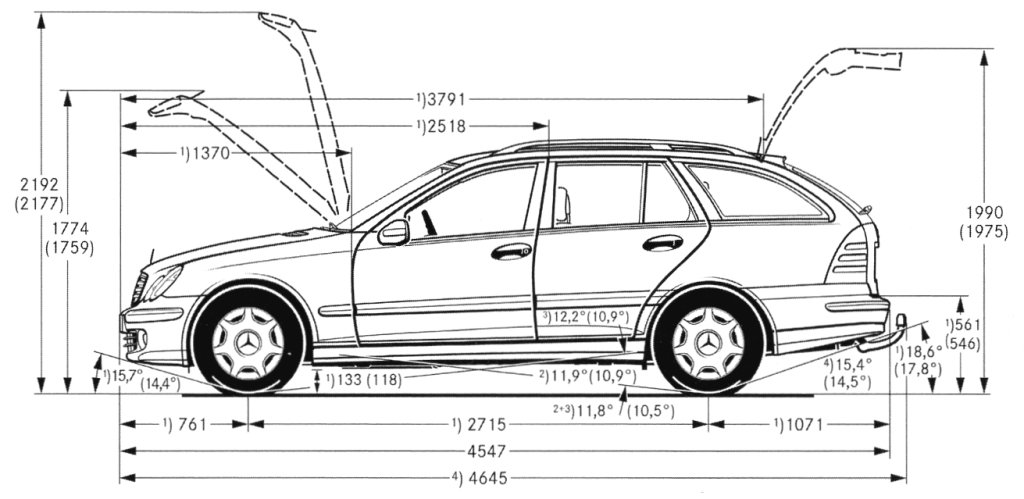
\includegraphics[width=0.95\textwidth]{images/S203_Seitenansicht}
	\caption{Side view diagram of a Mercedes-Benz CLC S203 AMG}
	\label{fig:car-sideview}
\end{figure}

%-----------------------------------------------------------------
\subsection{Programming the Controller}
The first need we need to do is to define some of the physical parameters of the system defined in table~\ref{tab:parameters}, this is shown in snippet~\ref{sn:physical} below:
\begin{lstlisting}[language=matlab, label=sn:physical, caption=Physical parameters for the model]
%% Parameters
% Reference angle
r = 0.25;
% Initial condition in degree
phi_0 = r + 0.1;
% Velocity in meters per second
V = 3.0;
% Example for Mercedes-Benz CLC S203 AMG in meters
L1 = 2.715;
L2 = 1.169;
L3 = 1.2;
\end{lstlisting}

As discussed in \cref{sec:intro-msct}, the eigenvalues of the system matrix, $A$, (equal to the poles of the transfer function) determine stability. In our system \eqref{eq:controler-system} we see that $A$ is positive; thus the system is unstable. The parameters to model the controller are defined in snippet~\ref{sn:model} below:
\begin{lstlisting}[language=matlab, label=sn:model, caption=Basic parameters to model the controller, firstnumber=13]
%% Model
A = V/L3;
B = V/L1*(1+L2/L3);
C = 1;
D = 0;
\end{lstlisting}

One of the first things we want to do is analyse whether the open-loop system (without any control) is stable. To observe what happens to this unstable system when there is a non-zero initial condition, we define the state space using \inline{sys = ss(A,B,C,0)} and then we simulate the output time response $y(t)$ of dynamic system with input $u(t)$ using the function \inline{lsim()}. This implementation can be seen in snippet~\ref{sn:open-loop} below:
\begin{lstlisting}[language=matlab, label=sn:open-loop, caption=Method to calculate open-loop response to non-zero initial condition, firstnumber=20]
%% Calculate open-loop response to non-zero initial condition

% Time in seconds
t = 0:0.01:10;
% Input
u = zeros(size(t))*r;
% Create state space object
sys = ss(A,B,C,0);

% Calculate open-loop response to non-zero initial condition
[y,t,x] = lsim(sys,u,t,phi_0);

% Plot the response
figure(1)
	plot(t,y)
	hold on
	plot(t,u)
	str_num = num2str(phi_0);
	str = strcat('Open-Loop Response to Non-Zero Initial Condition \phi_0=', str_num);
	title(str)
	xlabel('Time (sec)')
	ylabel('\phi (rad)')
	legend('Open-loop response', 'Reference')
	hold off
\end{lstlisting}

In figure \ref{fig:curve-open-loop} below we can see the uncontrolled behaviour of the system when there are no closed-loop poles (i.e., open-loop response). It's remarkable how quickly the jackknifing phenomenon occurs.
\begin{figure}[H]
	\centering
	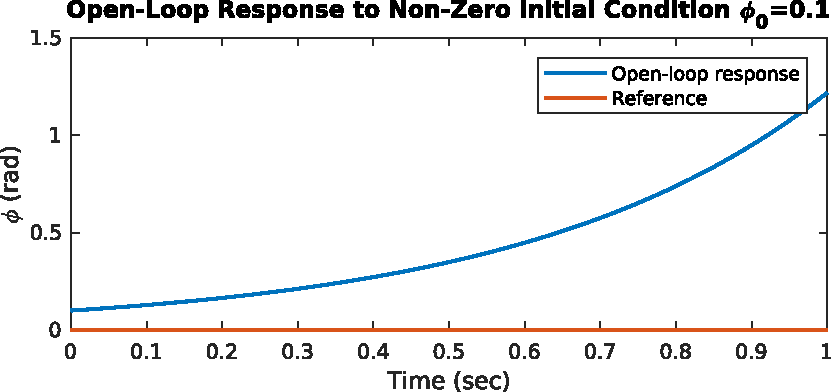
\includegraphics[width=0.7\textwidth]{images/curve-open-loop}
	\caption{Open-Loop response to non-zero initial condition driving backwards with a trailer}
	\label{fig:curve-open-loop}
\end{figure}

It is also worth noting that just as we expected from \eqref{eq:stability}, when $V < 0$ (using \inline{V = -3.0;} for instance) the system is stable, as seen in figure~\ref{fig:curve-open-loop-stable} below. In the figure, it can be clearly seen how when the car moves forward, the angle $\phi$ is corrected in a matter of seconds and then trailer flawlessly follows the car.
\begin{figure}[H]
	\centering
	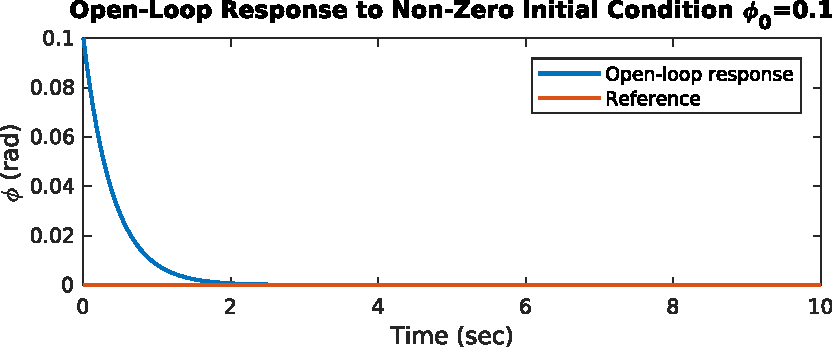
\includegraphics[width=0.73\textwidth]{images/stable-open-loop}
	\caption{Open-Loop response to non-zero initial condition driving forwards with a trailer}
	\label{fig:curve-open-loop-stable}
\end{figure}

%----------------------------------
Now that we know how the system behaves when there is no actual controller, let's see what happens when we introduce a closed-loop pole to control the system. We will work with several reference trajectories (discussed in \cref{sec:curves}) to see how the controller can handle different scenarios.

The major difference between this method and the previous one is that we now  build the controller for the system using a pole placement approach and assuming we have a full-state feedback system, meaning that all state variables are known to the controller at all times.

We use the function \inline{place()} to find the state-feedback gain, $K$, which will provide the desired closed-loop poles. Then we define the state space using \inline{sys_cl = ss(A-B*K,B,C,0);} and simulate the output time response $y(t)$ of dynamic system with input $u(t)$ using the function \inline{lsim()}, as seen in snippet~\ref{sn:closed-loop}.

One may see that we use a $\bar{N}$ factor in the calculation of the time response. We use the function \inline{rscale(sys,K)} to compute the desired $\bar{N}$ like presented in \cref{sec:controllerdesign}.

\begin{lstlisting}[language=matlab, label=sn:closed-loop, caption=Method to calculate closed-loop response to non-zero initial condition, firstnumber=44]
%% Calculate closed-loop response to non-zero initial condition

% Time in seconds
t = 0:0.01:60;
% Inputs
u = curve1(t, 0.35); % Standard curve
% u = curve2(t, 0.4); % U turn
% u = curve3(t, 0.65); % Sharp curve
% u = curve4(t, 0.4); % S shape

% Apply pole placement
K = place(A,B,-0.73);
% State space
sys_cl = ss(A-B*K,B,C,0);
% Calculate scaling factor
Nbar = rscale(sys,K);

% Calculate closed-loop response to non-zero initial condition
[y_cl,t,x_cl] = lsim(sys_cl,Nbar*u,t,phi_0);

% Plot the response
figure(2)
	plot(t,y_cl)
	hold on
	plot(t,u)
	str = strcat('Closed-Loop Response to Non-Zero Initial Condition \phi_0=', str_num);
	title(str)
	xlabel('Time (sec)')
	ylabel('\phi (rad)')
	legend('Closed-loop response', 'Reference')
	hold off
\end{lstlisting}

This implementation of a controller is the one previously illustrated in figure~\ref{fig:gain-schedule}.

%-----------------------------------------------------------------
\subsection{Controlling the Trailer on Different Curves}\label{sec:curves}
In this part we will see how the controller performs in terms of reaction time and fidelity with different trajectories. In particular we will work with (a) a short sharp curve, (b) a $U$ turn, and (c) an $S$-shaped curve.

%----------------------------------
\subsubsection*{Standard Curve}
In figure~\ref{fig:curve1a} we can see the shape of the trajectory followed by the car-trailer system, and in figure~\ref{fig:curve1b} we can see how the response of the controller to the input trajectory (defined in snippet~\ref{sn:curve1b}).

\begin{figure}[H]
	\centering
	\subfloat[Diagram of the curve]{%
		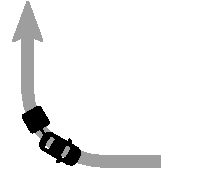
\includegraphics[height=0.2\textwidth]{images/curve1-diagram}%
		\label{fig:curve1a}%
		}%
	\hspace{0.5cm}%
	\subfloat[Closed-loop response of the controller]{%
		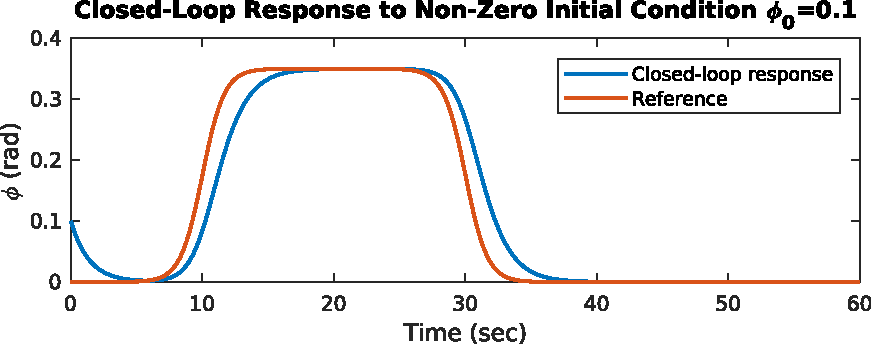
\includegraphics[height=0.25\textwidth]{images/control1-plot}%
		\label{fig:curve1b}%
		}%
	\caption{Diagram and control of the car-trailer system in a short, sharp curve}
\end{figure}

\begin{lstlisting}[language=matlab, label=sn:curve1b, caption=Function used to simulate a standard curve]
function [ x ] = curve1( t, height)
    steep = 2;
    n = length(t);

    x_1 = logistic(height, steep, linspace(-6,6,floor(n/3)), 0);
    x_2 = flip(x_1);

    x = [ x_1 height x_2 zeros(1,floor(n/3)) ];
end
\end{lstlisting}

This curve, along with a straight line, are the basis of basically all possible trajectories a car-trailer system can make whilst parking.

%----------------------------------
\subsubsection*{$U$-Turn Curve}
A $U$ turn simply consists on steering the wheel a longer time to the standard curve pr

In figure\ref{fig:curve2a} we can see the shape of the trajectory followed by the car-trailer system, and in figure~\ref{fig:curve2b} we can see how the response of the controller to the input trajectory (defined in snippet~\ref{sn:curve2}).

\begin{figure}[H]
	\centering
	\subfloat[Diagram of the curve]{%
		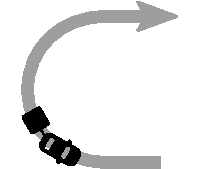
\includegraphics[height=0.2\textwidth]{images/curve2-diagram}%
		\label{fig:curve2a}%
		}%
	\hspace{0.5cm}%
	\subfloat[Closed-loop response of the controller]{%
		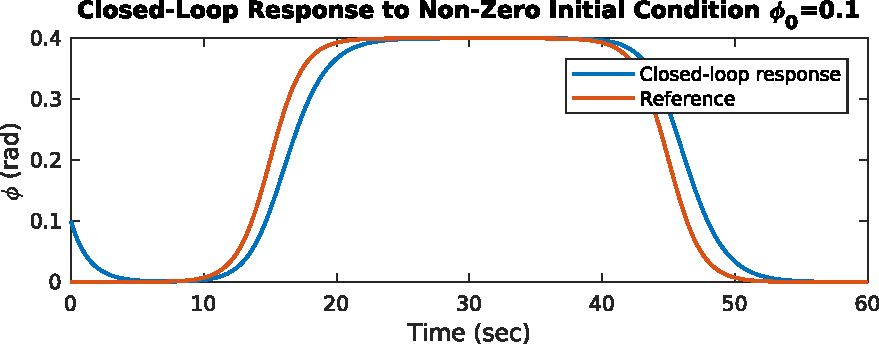
\includegraphics[height=0.25\textwidth]{images/control2-plot}%
		\label{fig:curve2b}%
		}%
	\caption{Diagram and control of the car-trailer system in a $U$ turn}
\end{figure}
\begin{lstlisting}[language=matlab, label=sn:curve2, caption=Function used to simulate a $U$ turn]
function [ x ] = curve2( t, height)
	steep = 2;
	n = length(t);

	x_1 = logistic(height, steep, linspace(-6,6,floor(n/2)), 0);
	x_2 = flip(x_1);

	x = [x_1 height x_2];
end
\end{lstlisting}

%----------------------------------
\subsubsection*{Short, Sharp Curve}
In figure~\ref{fig:curve3a} we can see the shape of the trajectory followed by the car-trailer system, and in figure~\ref{fig:curve3b} we can see how the response of the controller to the input trajectory (defined in snippet~\ref{sn:curve3b}).

\begin{figure}[H]
	\centering
	\subfloat[Diagram of the curve]{%
		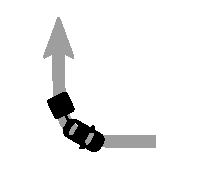
\includegraphics[height=0.2\textwidth]{images/curve3-diagram}%
		\label{fig:curve3a}%
		}%
	\hspace{0.5cm}%
	\subfloat[Closed-loop response of the controller]{%
		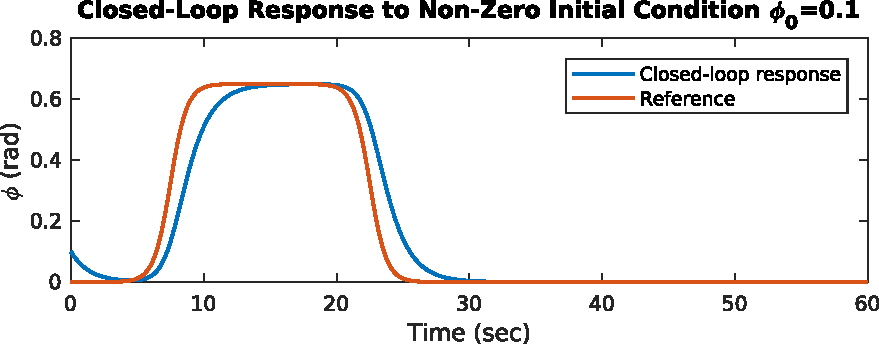
\includegraphics[height=0.25\textwidth]{images/control3-plot}%
		\label{fig:curve3b}%
		}%
	\caption{Diagram and control of the car-trailer system in a short, sharp curve}
\end{figure}

\begin{lstlisting}[language=matlab, label=sn:curve3b, caption=Function used to simulate a short sharp curve]
function [ x ] = curve1( t, height)
	steep = 2;
	n = length(t);

	x_1 = logistic(height, steep, linspace(-6,6,floor(n/4)), 0);
	x_2 = flip(x_1);

	x = [ x_1 height x_2 zeros(1,floor(n/2)) ];
end
\end{lstlisting}

%----------------------------------
\subsubsection*{$S$-Shaped Curve}
In figure~\ref{fig:curve4a} we can see the shape of the trajectory followed by the car-trailer system, and in figure~\ref{fig:curve4b} we can see how the response of the controller to the input trajectory (defined in snippet~\ref{sn:curve4}).

\begin{figure}[H]
	\centering
	\subfloat[Diagram of the curve]{%
		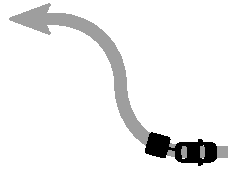
\includegraphics[height=0.2\textwidth]{images/curve4-diagram}%
		\label{fig:curve4a}%
		}%
	\hspace{0.5cm}%
	\subfloat[Closed-loop response of the controller]{%
		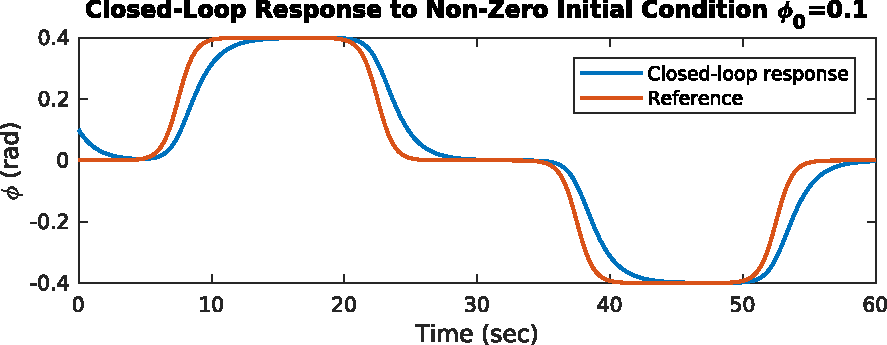
\includegraphics[height=0.25\textwidth]{images/control4-plot}%
		\label{fig:curve4b}%
		}%
	\caption{Diagram and control of the car-trailer system in a $S$-shaped curve}
\end{figure}
\begin{lstlisting}[language=matlab, label=sn:curve4, caption=Function used to simulate an $S$-shaped curve]
function [ x ] = curve3( t, height )
	steep = 2;
	n = length(t);

	x_1 = logistic(height, steep, linspace(-6,6,floor(n/4)), 0);
	x_2 = flip(x_1);
	x_3 = [ x_1 x_2 ];
	x_4 = -x_3;

	x = [ x_3 0 x_4 ];
end
\end{lstlisting}

%-----------------------------------------------------------------
\subsection{Issues with the Model}

Main problem about this model is that it is a continuous model which cannot be implemented on a chip without modification. One needs to discretise it. There are several options to do so, each having advantages and disadvantages. One could think about creating a continuous model with continuous model and afterwards doing the discretisation. Another approach would be just to discretise the model and create a discrete version of the controller. These two approaches are not equivalent. Obviously, the first one is more powerful because it will provide insights into the system behaviour for all times $t$ whereas the second one only yield information for the sampling instances $kT$. The advantage of this method is that it is easier to apply.

Another problem is that the model is obtained by linearisation about the operation point $\SI{0}{\degree}$. One improvement would be to use a gain-scheduling controller which is also linear. This group of controller is often applied to nonlinear models. It selects the gain according to some strategy. This strategy e.g. can be time-varying or depended on the state of the system. In our case we would prefer a state dependent scheduler since our system behaves linearly in small regions for different operating points: $[-\SI{40}{\degree},\SI{40}{\degree}]$. For implementation we would need to linearise the model for all these operating points with a sufficient small step size. However, to show feasibility and solvablity of the problem it is sufficient to linearise about one operation point. 

%-----------------------------------------------------------------
%	ALTERNATIVE IMPLEMENTATIONS
%	!TEX root = ./../main.tex
%-----------------------------------------------------------------



\section{Alternative Controlling Methods}

We have used alternative methods that do not use control theory in order to make the trailer follow the path that we want. These methods focus on different heuristics to determine which $\delta$ we have to choose in order to go through the desired path. The first method thinks on a function to optimise in order to be as close as possible to the desired path and as close as possible to the critical point $\phi = 0$. The second one aims to replicate the strategy of expert trailer drivers that have a lot of experience in our problem.\\

\subsection{Optimisation-based control}

Using the model derived in \cref{kinem}, we aim to move our trailer in a straight path. Of course, our straight path will start with an angle $\phi \neq 0$, which tries to resemble a situation where we are trying to go backwards but the trailer starts to bend due to some imperfection of the ground/wheels.\\

We will assume, without loss of generality, that the centre of mass of our car starts at the origin. As we want the car to go straight, we will make the car go backwards in the $x$ axis, and the car will start aligned with this axis. On the other hand, the trailer will not start aligned with the $x$ axis (if not, the solution would be trivial, setting $\delta = 0$ the whole time would solve the problem). Our aim is to go through the $x$ axis during a quantity of time $T$. However, what does going through the $x$ axis mean?
We will set a tolerance $\Delta y$, and if at time $T$ the trailer is at a distance from the $x$ axis lower than $\Delta y$, we will take it a success. In mathematical terms, we have to decide a function $\delta(t)$, for $0\leq t \leq T$, such that $\abs{y(T)} < \Delta y$ and $\abs{\phi} < \phi_{crit}$, where $\phi_{crit}$ is the critical jackknifing angle.\\

To find the \textit{steering function} $\delta(t)$, we will use a brute force method. We will split the interval $[0, T]$ into $n$ interval times of length $T/n$. At the beginning of each interval, we will choose which is the $\delta$ that puts the trailer in the best possible configuration at the end of the interval. We will simulate the trajectory of the whole system in order to decide how good is a choice of $\delta$. In addition, we have to determine when is a configuration better than another one. To do this, we have chosen a cost function. The cost function that we have chosen depends on the angle $\phi$ and the distance from the $x$ axis, $\abs{y}$. We have taken:
\begin{align}
    \operatorname{cost}_{\alpha}(y, \phi) = y^2+\alpha\phi^2 
\end{align}
The cost function defined above depends on a parameter, $\alpha$. The higher $\alpha$ is, the more we are interested in keeping the trailer aligned. The lower $\alpha$ is, the more we are interested in keeping the car on the path regardless of the trailer. Then, $\alpha$ is a parameter that needs to be tuned in every different geometrical configuration. \\

Now that we have our cost function defined, our method to find the steering function $\delta(t)$ works as follows: for each of the time intervals that we have divided our time into, at the beginning of the interval we choose the $\delta$ that minimises $\operatorname{cost}_{\alpha}$ at the end of the interval. The way to find the optimal $\delta$ is by means of brute force: We search in a grid of angles in the interval $[-\delta_{max}, \delta_{max}]$ and number of elements $n_{\delta}$. With this method, the output function $\delta(t)$ is a piecewise function that at every time interval has a constant value.\\

One of the main drawbacks of the method is that, given a time $T$, the method depends on three parameters that we do not know which value they should have a priori: $n$, $n_\delta$ and  $\alpha$. One could argue that, the higher the $n$, the more chances that the method can find the solution. However, this is far from the truth. The main problem is that method tries to optimise the configuration of the system at the next time step: however, this does not in principle guarantee that this configuration will be optimal after that time step. For this reason, having a very large $n$ can be considered very elitist, thus not allowing us to find the proper steering function. These kind of elitist searches are usually known as greedy algorithms.\\

We have implemented the previous method in $C$, using the analytical expressions for the circular paths of the points in the car and using a Runge--Kutta--Fellberg 78 method to integrate the differential equation for $\phi$. We have used sensible data for the length and width of each of the elements of the system.  Our aim would be to keep the system going straight for a given amount of time $T$. When $T$ is large enough ($T\approx 10$ seconds), the system is very hard to be controlled in the whole interval. We have tried many values of $\alpha$, $n$ and $n_\delta$, but they all fail when given a sufficiently large amount of time $T$.\\


We think that this method does not work due to the fact that the method only focuses on optimising the next time step. This is a main drawback, as not only it forgets about time steps that follow the next one, but it may also be that optimising the next time step is bad for the long run. In terms of optimisation, we can say that we are constantly being elitist, and this is usually not the best strategy when we want to optimise complicated functions. For this reason, the next method is a little bit more exploratory, that is, it does not always look at the best solution in its neighbourhood, but in the long run it performs better.\\

% \subsection{Experienced control}
\subsection{Steering-based control}
In this section we describe the method to get the trailer from one point to another by using steering strategies that reassemble the ones used by experienced drivers.\\

The method is made up of iteratively-repeated steering steps that we have defined as a \textit{manoeuvre}. A \textit{manoeuvre} consists in two steps: the first one, to bend the trailer into the right direction, and the second one, to move the car towards the desired end.\\

We will call the first part of the \textit{manoeuvre} \emph{trailer facing}. The way to perform \emph{trailer facing} is the following. Assume that if you had to go from the beginning point to the final point \textit{without} a trailer you would have to take $\delta > 0$ to go upwards. In this case, the trailer would quickly face the opposite direction, it would go downwards. In this way, in order get the trailer facing to the right direction, we need to start by taking $\delta < 0$. This is counter-intuitive: we are moving in the wrong direction. We move into the wrong direction in order to face the trailer into the right direction. The problem of starting to move into the right direction is that the trailer faces the wrong direction and then we would have to correct it afterwards. This later correction would not allow us to achieve the final point.\\

\begin{figure}[H] 
    \centering
    \subfloat[Initial situation]{%
        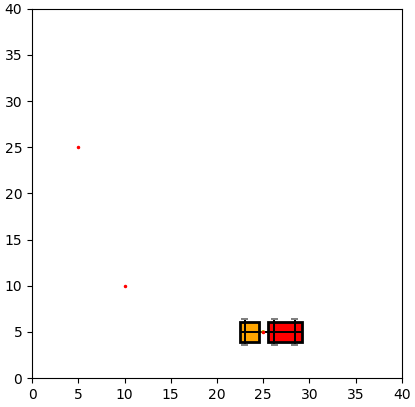
\includegraphics[width=0.45\textwidth]{images/pic1.png}%
        \label{fig:pic1a}%
        }%
    \hspace{0.5cm}%
    \subfloat[Situation after the first trailer facing]{%
        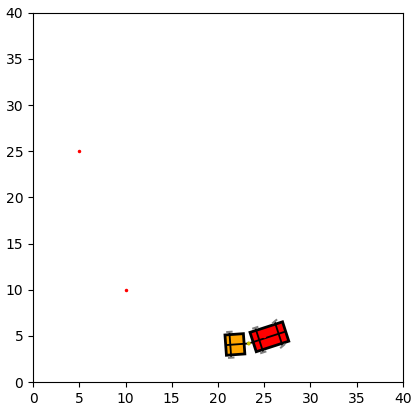
\includegraphics[width=0.45\textwidth]{images/pic2.png}%
        \label{fig:pic1b}%
        }%
    \caption{Trailer facing}
\end{figure}

In the picture above, we can see an example of the \emph{trailer facing} working. The initial conditions are the ones shown in \ref{fig:pic1a}, and our aim is to arrive to red point at (10, 10). If we were not using a trailer, we would steer the car such that it went towards higher $y$. However, as we can see in \ref{fig:pic1b} we are doing the exact opposite: we are going to even lower $y$. Once we have done this, the trailer is properly faced: when we go to the red point, the trailer will not jackknife as easily as if we had gone to the red point when we were in \ref{fig:pic1a}. This is because, when going to the red point, the trailer will bend to the opposite direction after the trailer facing, thus having to cross through the point $\phi = 0$.

However, we still have to decide what having a proper facing means. We will set a $\phi_{max}$ at which we end the trailer facing. This $\phi_{max}$ will not be static. If we are far away from the end point, we will set a high $\phi_{max}$, as we want to bend more. If we are close to the point, we will set a lower $\phi_{max}$, as we do not need to bend that much. In all cases, when $\phi = \phi_{max}$ we will end the trailer facing and start the car facing.\\


Once we have the trailer facing into the right direction, we start the second part of the manoeuvre: car facing. In this part, we act as if we had no trailer and we choose the $\delta$ such that the car goes to the end point. We do this until the trailer is faced into the wrong direction, and then we go back to the first part of the \textit{manoeuvre} again.\\

\begin{figure}[H] 
    \centering
    \subfloat[Faced trailer]{%
        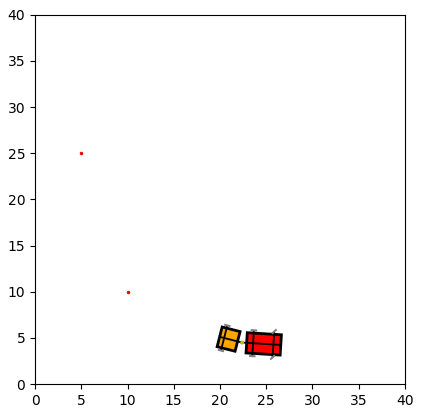
\includegraphics[width=0.30\textwidth]{images/picCF1.png}%
        \label{fig:piccf1a}%
        }%
    \subfloat[Trailer with $\phi \approx 0$]{%
        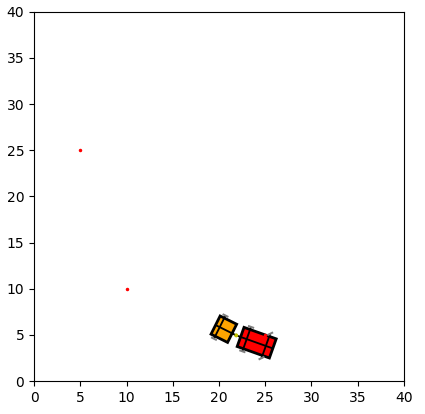
\includegraphics[width=0.30\textwidth]{images/picCF2.png}%
        \label{fig:piccf1b}%
        }%
    \subfloat[Trailer wrongly faced]{%
        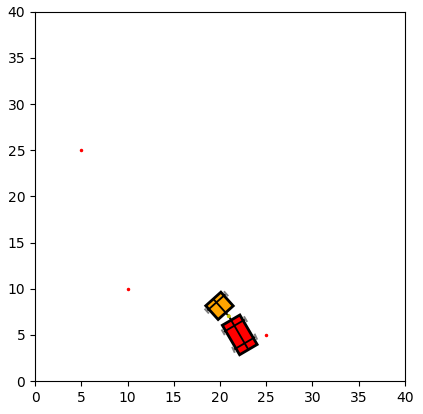
\includegraphics[width=0.30\textwidth]{images/picCF3.png}%
        \label{fig:piccf1c}%
        }%
    \caption{Trailer facing}
\end{figure}

In the picture shown above we can see how the trailer goes from being properly faced to a facing that if goes on it can cause a jackknife. In this picture we can see how the car gets closer to the red point ($y$ grows), and the price to pay is the misalignment of the trailer. Once it is enough misaligned, we will start with the trailer facing.\\

So far, we have just told about choosing $\delta > 0$ or $\delta < 0$, but we haven't specified which $\delta$ to use. In order to make the model more realistic, $\delta(t)$ will be a continuous function. That is, we are allowed a maximum variation of angle $\Delta \delta$ every time step $\Delta t$. That is, the maximum steering speed of the driver is $\Delta \delta / \Delta t$. For this reason, we can't always aim at the optimal $\delta$ every time step, as, if we were steering at $\delta_0$ at the last step, we can only aim at the best $\delta$ in $(\delta_0 -\Delta \delta, \delta_0 + \Delta \delta)$. How do we choose this best $\delta$? We use the discretised differential equation. Ideally, if we want to make an increase in $\phi$ of $\Delta \phi$, we have to take the $\delta$ satisfying the following equality:
\begin{align}
    \frac{\Delta \phi}{\Delta t} = - \frac{V}{L_{3}} \sin \phi - \frac{V}{L_{1}} \tan \delta \qty( 1 + \frac{L_{2}}{L_{3}} \cos \phi )
\end{align}
Which is given by:
\begin{align}
    \delta = \arctan\frac{-L1\cdot(\Delta \phi\cdot L3-\sin\phi\cdot\Delta t\cdot V)}{\Delta t\cdot V(L3+L2\cdot \cos\phi)} 
\end{align}
However, we cannot always choose this $\delta$, as this $\delta$ might not be in the interval $(\delta_0 -\Delta \delta, \delta_0 + \Delta \delta)$. For this reason, if $\delta > \delta_0 + \Delta \delta$, we choose $\delta = \delta_0 + \Delta \delta$. If $\delta < \delta_0 - \Delta \delta$, we choose $\delta = \delta_0 - \Delta \delta$.\\

Of course, we still need a criteria to decide which is the $\Delta \phi$ value that we want to attain. Different choices can be made, but we have chosen just to focus on the direction, not thinking about the actual value of $\phi$, for simplicity. If we want the trailer to go towards negative $\phi$ values, we will just set $\Delta \phi = -1$, and if we want it to go towards positive values we will choose $\Delta \phi = 1$. The decision of going towards positive and negative values is made upon the trailer facing or car facing criteria.



\subsection{Comparison of the two methods}

% As we have said before, the first method works by constantly looking for the optimal solution at the next time step. We have checked that this method does not work when aiming at a sufficiently large amount of time. The main drawback of this method is that the optimal configuration in the next step might not be good in the long run. On the other hand, the experienced method does not have this problem. Sometimes, it starts bending to the opposite side and getting much worse locally. However, this allows it to get better globally.

As we have said before, the first method works by constantly looking for the optimal solution at the next time step. We have checked that this method does not work when aiming at a sufficiently large amount of time. The main drawback of this method is that the optimal configuration in the next step might not be good in the long run. On the other hand, the steering-based method does not have this problem. Sometimes, it starts bending to the opposite side and getting much worse locally. However, this allows it to get better globally.



%---------------------The main drawback of this method is that the optimal configuration in the next step might not be good in the long run. On the other hand, the experienced method does not have this problem. Sometimes, it starts bending to the opposite side and getting much worse locally. However, this allows it to get better globally.--------------------------------------------
\subsection{Further improvements}

From experience, it is hard to make the trailer go straight, even when the axles are aligned (due to the fact that alignment is not perfect, and the equilibrium point is unstable). To model this, we can introduce some perturbations in the angle of the trailer. After doing an integration step, we will add some uniform noise to the $\phi$ angle, with expectation value $0$. We choose this kind of noise because a priori we do not have any preferred direction of the perturbations. The interval $(-r, r)$ of the uniform random variable that models the noise will have a fixed length $2r$, which has been chosen small (but way bigger than $10^{-16}$, which is the \textit{numerical noise} given by the finite decimals of the representation of the double precision numbers). The randomisation just affects to the kinematics, as the method to control the trailer is based on the same criteria. However, every trajectory of the trailer is different, due to the random effects. As, with $r = 0.025$, the trailer finishes successfully the path, this means that our method is robust and could be applied to ground with some slippery.\\

To illustrate that every simulation is different, and although the method is the same, it provides different steering functions $\delta(t)$, we have plotted in two runs of the method how $\phi$ and $\delta$ vary over time.

\begin{figure}[H] 
    \centering
    \subfloat[Comparison of $\phi(t)$ evolution]{%
        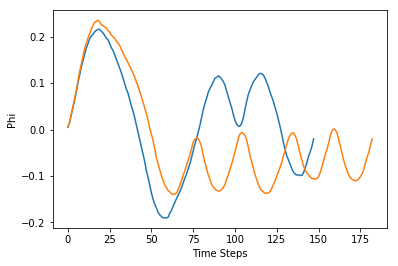
\includegraphics[width=0.45\textwidth]{images/phis.png}%
        \label{fig:phis}%
        }%
    \hspace{0.5cm}%
    \subfloat[Comparison of steering functions $\delta(t)$]{%
        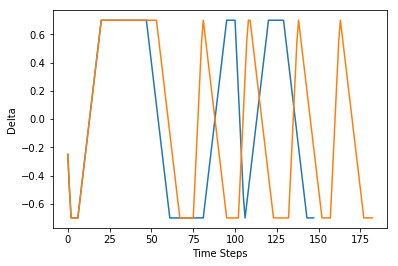
\includegraphics[width=0.45\textwidth]{images/deltas.png}%
        \label{fig:deltas}%
        }%
    \caption{Variation of the angles in different runs of the algorithm}
\end{figure}

We can see that one of the methods (blue) finishes earlier. Although having very different paths, they both terminate successfully. We can see that the initial conditions are similar but at some point they start to differ. After they start to differ, the steering functions change, as they adapt to the current $\phi$ value. As the steering starts to differ, this makes the path change more and more, ending with very different trajectories.
%-----------------------------------------------------------------
%	CONCLUSIONS
%	!TEX root = ./../main.tex
%-----------------------------------------------------------------
\section{Conclusions}

In the previous sections we have three different approaches to implement a controller to aid the driver in the process of parking with a trailer attached to their car:
\begin{itemize}
    \item State space control (using MATLAB).
    \item Optimisation-based control (using C).
    \item Steering-based control (using Python).
\end{itemize}

Except the optimisation-based control, we showed that all of the models are viable options for control with their own advantages and disadvantages.

\bigskip
We think that as an improvement and further development of our work it would be interesting to test our results. We could consider a simulation or even a real miniature car with a trailer using LEGO MINDSTORMS NXT (or similar) using MATLAB's Simulink or Python's \inline{nxt-python} library.


%-----------------------------------------------------------------
%	BIBLIOGRAPHY
%-----------------------------------------------------------------

\nocite{Nilsson2013}

\printbibliography[heading=bibintoc]
% \setcounter{secnumdepth}{0}
% \section{References}
% \printbibliography[title={Articles}, type=article, heading=subbibliography]
% \printbibliography[title={Books}, type=book, heading=subbibliography]
% \printbibliography[title={Websites}, type=online , heading=subbibliography]
% \printbibliography[title={Basic}, keyword=basic , heading=subbibliography]

\end{document}
